\documentclass{beamer}
\usepackage[utf8]{inputenc}

\usetheme{Boadilla}
\usecolortheme{lily}
\usepackage{amsmath,amssymb,amsfonts,amsthm}
\usepackage{mathtools}
\usepackage{txfonts}
\usepackage{tkz-euclide}
\usepackage{listings}
\usepackage{adjustbox}
\usepackage{array}
\usepackage{tabularx}
\usepackage{lmodern}
\usepackage{gvv}
\usepackage{circuitikz}
\usepackage{tikz}
\usepackage{graphicx}

\setbeamertemplate{footline}
{
  \leavevmode%
  \hbox{%
  \begin{beamercolorbox}[wd=\paperwidth,ht=2.25ex,dp=1ex,right]{author in head/foot}%
    \insertframenumber{} / \inserttotalframenumber\hspace*{2ex} 
  \end{beamercolorbox}}%
  \vskip0pt%
}

\usepackage{tcolorbox}
\tcbuselibrary{minted,breakable,xparse,skins}




\providecommand{\nCr}[2]{\,^{#1}C_{#2}} % nCr
\providecommand{\nPr}[2]{\,^{#1}P_{#2}} % nPr
\providecommand{\mbf}{\mathbf}
\providecommand{\pr}[1]{\ensuremath{\Pr\left(#1\right)}}
\providecommand{\qfunc}[1]{\ensuremath{Q\left(#1\right)}}
\providecommand{\sbrak}[1]{\ensuremath{{}\left[#1\right]}}
\providecommand{\lsbrak}[1]{\ensuremath{{}\left[#1\right.}}
\providecommand{\rsbrak}[1]{\ensuremath{{}\left.#1\right]}}
\providecommand{\brak}[1]{\ensuremath{\left(#1\right)}}
\providecommand{\lbrak}[1]{\ensuremath{\left(#1\right.}}
\providecommand{\rbrak}[1]{\ensuremath{\left.#1\right)}}
\providecommand{\cbrak}[1]{\ensuremath{\left\{#1\right\}}}
\providecommand{\lcbrak}[1]{\ensuremath{\left\{#1\right.}}
\providecommand{\rcbrak}[1]{\ensuremath{\left.#1\right\}}}
\theoremstyle{remark}
\newcommand{\sgn}{\mathop{\mathrm{sgn}}}
\providecommand{\abs}[1]{\left\vert#1\right\vert}
\providecommand{\res}[1]{\Res\displaylimits_{#1}} 
\providecommand{\norm}[1]{\lVert#1\rVert}
\providecommand{\mtx}[1]{\mathbf{#1}}
\providecommand{\mean}[1]{E\left[ #1 \right]}
\providecommand{\fourier}{\overset{\mathcal{F}}{ \rightleftharpoons}}
%\providecommand{\hilbert}{\overset{\mathcal{H}}{ \rightleftharpoons}}
\providecommand{\system}{\overset{\mathcal{H}}{ \longleftrightarrow}}
	%\newcommand{\solution}[2]{\textbf{Solution:}{#1}}
%\newcommand{\solution}{\noindent \textbf{Solution: }}
\providecommand{\dec}[2]{\ensuremath{\overset{#1}{\underset{#2}{\gtrless}}}}
\newcommand{\myvec}[1]{\ensuremath{\begin{pmatrix}#1\end{pmatrix}}}
\let\vec\mathbf

\lstset{
%language=C,
frame=single, 
breaklines=true,
columns=fullflexible
}

\numberwithin{equation}{section}

\lstset{
  language=Python,
  basicstyle=\ttfamily\small,
  keywordstyle=\color{blue},
  stringstyle=\color{orange},
  numbers=left,
  numberstyle=\tiny\color{gray},
  breaklines=true,
  showstringspaces=false
}

\title{Problem 3.0.23}
\author{ee25btech11023-Venkata Sai}

\date{\today} 
\begin{document}

\begin{frame}
\titlepage
\end{frame}

\section*{Outline}
\begin{frame}
\tableofcontents
\end{frame}

\section{Problem}

\begin{frame}
\frametitle{Problem}
Let $x_1 = 3.5$, $x_2 = 7.5$ and $x_3 = 5.2$ be observed values of a random sample of size 
three from a population having uniform distribution over the interval $(\theta, \theta + 5)$, 
where $\theta \in (0, \infty)$ is unknown and is to be estimated. Then which of the 
following is NOT a maximum likelihood estimate of $\theta$?

\begin{enumerate}
    \item 2.4
    \item 2.7
    \item 3
    \item 3.3
\end{enumerate}
\end{frame}
%\subsection{Literature}
\section{Solution}

\subsection{Representation}
\setcounter{section}{1}
\begin{frame}
\frametitle{Representation}
 For a random sample $x_1, x_2, \dots, x_n$ from a uniform distribution $U(\theta, \theta+5)$, the probability density function (PDF) for each observation is:

\begin{align}
f(x_i | \theta) = 
\begin{cases} 
\frac{1}{5}, & \theta < x_i < \theta + 5 \\
0, & \text{otherwise}
\end{cases}
\end{align}
The likelihood function $L(\theta)$ for the sample of size $n=3$ is the product of the individual PDFs:

\begin{align}
L(\theta) = \prod_{i=1}^{3} f(x_i | \theta) = 
\begin{cases} 
\left(\frac{1}{5}\right)^3 = \frac{1}{125} & \text{if } \theta \leq x_i \leq \theta + 5 \text{ for all } i \\ 
0 & \text{otherwise} 
\end{cases}
\end{align}

\end{frame}
\subsection{Constraints on $\theta$}
\begin{frame}
\frametitle{Constraints on $\theta$}
$\theta$ must be less than or equal to all observed values:
\begin{align}
\theta &\le \min(x_1, x_2, x_3) \\
\theta &\le 3.5 
\end{align}
Also the upper limit must be greater than or equal to all observed values, Hence
\begin{align}
\theta + 5 &\geq \max(x_1, x_2, x_3) \\
\theta + 5 &\geq 7.5 \\
\theta &\geq 7.5 - 5 \\
\theta &\geq 2.5 
\end{align}

\end{frame}

\begin{frame}
\frametitle{Calculation}
 Combining both the constraints, We get the range of $\theta$
 \begin{align}
     2.5 \leq \theta \leq 3.5
 \end{align}
 From the options,
 2.7, 3, 3.3 lies in range of $\theta$ but 2.4 doesn't.
 
 Hence 2.4 is NOT a maximum likelihood estimate of $\theta$.
 \end{frame}

\section{Plot}

\begin{frame}
\frametitle{Plot}
\begin{figure}
    \centering
    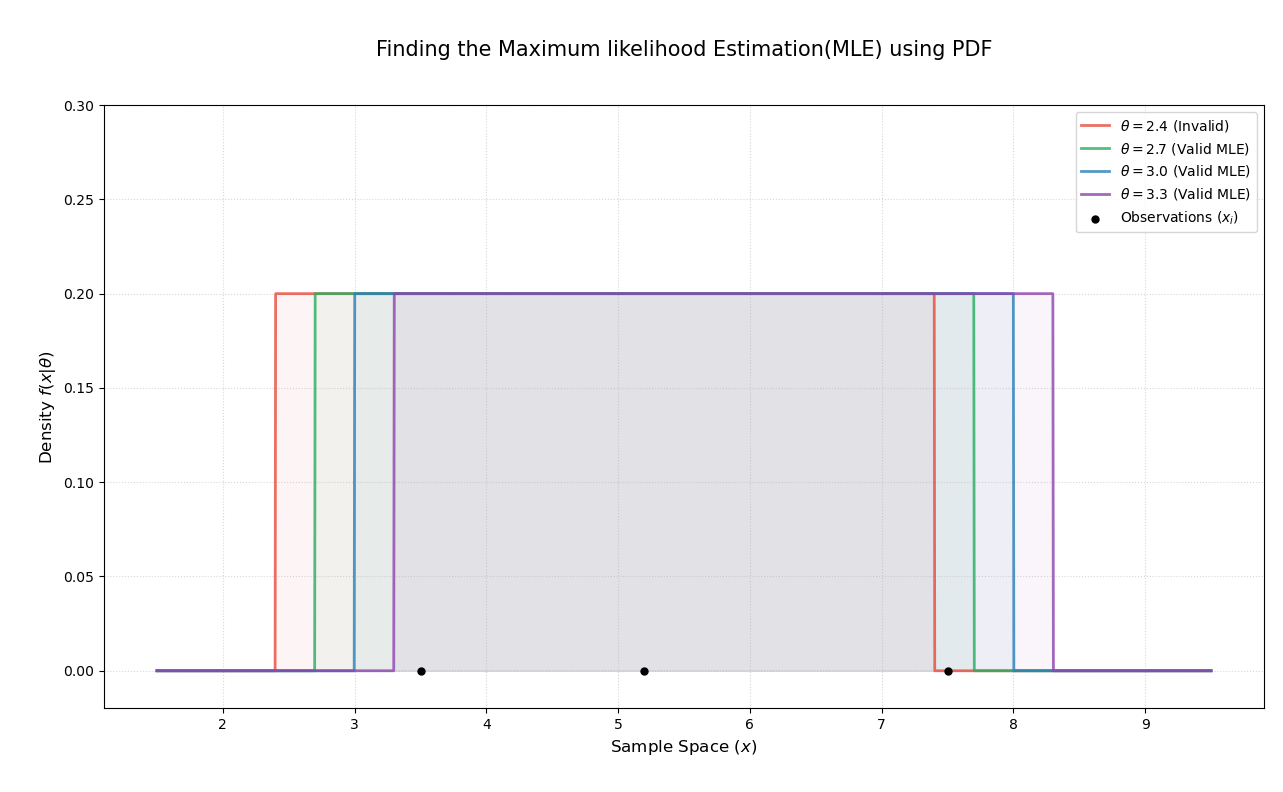
\includegraphics[width=0.9\linewidth]{figs/Fig1.png}
    \label{Figure 1}
\end{figure}
\end{frame}

\section{Python Code}
\begin{frame}[fragile]
\frametitle{Python Code for Plotting}
\begin{lstlisting}[language=Python]
import numpy as np
import matplotlib.pyplot as plt
from scipy.stats import uniform

# Setup figure
fig, ax = plt.subplots(figsize=(14, 8))

# Define our observed data
data = np.array([3.5, 5.2, 7.5])

# Define the candidate thetas to test and their colors
thetas =[2.4, 2.7, 3.0, 3.3]
colors = ['#e74c3c', '#27ae60', '#2980b9', '#8e44ad']

x = np.linspace(1.2, 9.8, 5000)

# Loop through, calculate validity, and plot using SciPy
for theta, color in zip(thetas, colors):



\end{lstlisting}
\end{frame}
 
\begin{frame}[fragile]
\frametitle{Python Code for Plotting}
\begin{lstlisting}[language=Python]

    is_valid = np.all((data >= theta) & (data <= theta + 5))

    status = "Valid MLE" if is_valid else "Invalid"
    dynamic_label = rf'$\theta = {theta}$ ({status})'

    # Calculate PDF using SciPy
    y = uniform.pdf(x, loc=theta, scale=5)

    # Plot the outline calculated by SciPy
    ax.plot(x, y, color=color, linewidth=2.2, alpha=0.9, label=dynamic_label)

    ax.fill_between(x, y, 0, color=color, alpha=0.08)

# Plot the observed data points
ax.scatter(data, [0, 0, 0], color='black', s=35, zorder=10,
           label=r'Observations ($x_i$)')



\end{lstlisting}
\end{frame}
\begin{frame}[fragile]
\frametitle{Python Code for Plotting}
\begin{lstlisting}[language=Python]
# Formatting
ax.set_title('Finding the Maximum likelihood Estimation (MLE) using PDF',
             fontsize=16, pad=25)
ax.set_xlabel(r'Sample Space ($x$)', fontsize=12)
ax.set_ylabel(r'Density $f(x|\theta)$', fontsize=12)

# Set axis limits
ax.set_ylim(-0.02, 0.30)

# Add a light dotted grid
ax.grid(True, linestyle=':', alpha=0.5)

# Add the legend
ax.legend(loc='upper right', framealpha=1.0, fontsize=10.5)

plt.tight_layout()
plt.show()
\end{lstlisting}
\end{frame}

\end{document}